\documentclass[]{report}

\voffset=-1.5cm
\oddsidemargin=0.0cm
\textwidth = 480pt

\usepackage{framed}
\usepackage{subfiles}
\usepackage{graphics}
\usepackage{newlfont}
\usepackage{eurosym}
\usepackage{amsmath,amsthm,amsfonts}
\usepackage{amsmath}
\usepackage{enumerate}
\usepackage{color}
\usepackage{multicol}
\usepackage{amssymb}
\usepackage{multicol}
\usepackage[dvipsnames]{xcolor}
\usepackage{graphicx}

\begin{document}

\subsection*{Operations Research - Tutorial Set Question 31 to 60}
%------------------%
\begin{enumerate}
	\setcounter{enumi}{30}

\item 
Find the backward-induction solutions of the following extensive form game.
\begin{figure}[h!]
	\centering
	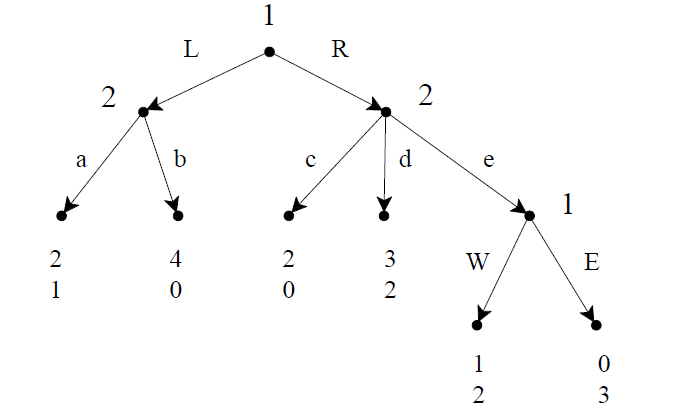
\includegraphics[width=0.45\linewidth]{Q31}
	
\end{figure}

%=========================%
%- Question 32


\item Solve the following game using Backward Induction. Express the game as a matrix game.

\begin{figure}[h!]
	\centering
	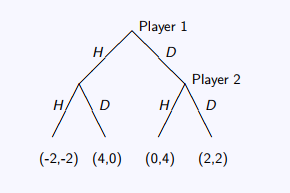
\includegraphics[width=0.4\linewidth]{Q32}
	
\end{figure}


%-----------------%
%- Schaum
\item \textbf{Construct a payoff matrix far the following game.}\\

\begin{itemize}
	\item Each of two supermarket chains proposes to 
	build a store in a rural region that is served by three towns. The distances between towns are 
	shown in the figure below.\begin{figure}[h!]
		\centering
		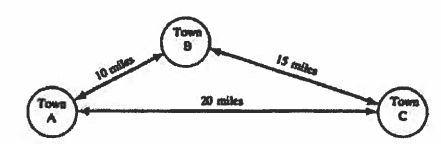
\includegraphics[width=0.45\linewidth]{Q35}
	\end{figure}
	
	\item Approximately 43 percent of the. regiions population live near town A, 33 
	percent live near town B. and 70 percent live near town C. 
	\item Because Chain 1 is larger and has 
	developed a better reputation than chain 2. chain 1 will control a majority of the business 
	whenever their situations are comparable. 
	\item 
	Both chains are aware of the other's interest in the region and both have completed marketing surveys that give identical projections.
	\item  If 
	both chains locate in the same town or equidistant from a town, chain 1 will control 65 percent of the business in that town. 
	\item
	If chain I 1 closer to a town than chain 2. chain I will control 90 mem of that towns business. 
	\item If chain 1 is farther from a town 
	than chain 2, it will still draw 40 percent of that town's business, The remaining business under all circumstances will go to chain 2. 
	\item Furthermore, both chains know that it is the policy of chain I not to locate in towns that are too small, and town C falls into this category. 
	
\end{itemize}
%-----------------%


\item \textbf{Cournot Equilibrium - Introduction to Duopolies}\\% Bonanno


Determine the Cournot-Nash Equilibrium of the following Duopoly Model.

\begin{itemize}
	
	\item
	
	\item
	
\end{itemize}

%-----------------%
\item Cournot 2


Determine the Cournot-Nash Equilibrium of the following Duopoly Model.

\begin{itemize}
	
	\item
	
	\item
	
\end{itemize}
%-----------------%
\item Cournot 3

Determine the Cournot-Nash Equilibrium of the following Duopoly Model.

\begin{itemize}
	
	\item
	
	\item
	
\end{itemize}

%-----------------%
\item \textbf{Bertrand Duopoly 1 (Identical Goods)}

%- Sporting Clay

Determine the Bertrand Equilibrium of the following Duopoly Model.

\begin{itemize}
	
	\item
	
	\item
	
\end{itemize}
%-----------------%
\item \textbf{Bertrand Duopoly 2 (Different Goods)}

%- Sporting Clay

Determine the Bertrand Equilibrium of the following Duopoly Model.

\begin{itemize}
	
	\item
	
	\item
	
\end{itemize}
%-----------------%
\item \textbf{Stackleberg Quantity Leadership Problem}
%- Lady


Determine the Stackleberg Equilibrium of the following Duopoly Model.

\begin{itemize}
	
	\item
	
	\item
	
\end{itemize}

%-----------------%
\item \textbf{Stackleberg : 2 Firm with Identical Goods}
%- Sporting Clay
Determine the Stackleberg Equilibrium of the following Duopoly Model.



 \item
 \begin{enumerate}[(a)]
 	\item Big O-notation is used to classify algorithms according to their relative complexity. Compare the complexity of algorithms of order $\mathrm{O}(\log n)$, $\mathrm{O}(n)$, $\mathrm{O}(n\log n)$, $\mathrm{O}(2^n)$and $\mathrm{O}(n!)$. Illustrate your answer with a sketch. 
 	\item Classify the Binary Search Tree algorithm using Big $\mathrm{O}$-notation. Justify your answer. 
 	\item Compare and contract Big O-Notation, Big Omega Notation and Big Theta Notation. 
 	
 	\item What is meant by Combinatorial Explosion? Why is it relevant for Binary Integer Problems? 
 	
 \end{enumerate}

%===================================%
% Question 60
\item \textbf{Algorithm Definition Questions}
\begin{multicols}{2}
	\begin{itemize}

		\item Knapsack Problem
		\item Provide illustrations / Examples
	\end{itemize}
\end{multicols}
 	



\end{enumerate}


\end{document}
